\documentclass[11pt]{article}
\usepackage{geometry}                
\geometry{letterpaper} 
\usepackage{graphicx}
\usepackage{amssymb}
\usepackage{epstopdf}
\usepackage{amsmath}
\usepackage[round]{natbib}
\DeclareGraphicsRule{.tif}{png}{.png}{`convert #1 `dirname #1`/`basename #1 .tif`.png}

\newcommand{\E}{\mathcal{E}}
 
\title{\vspace{-0.5in}Internal Note: The Casimir Force in a Micron-Scale Optical Trap Geometry}
\author{Noah Kurinsky}
%\date{}                                  

\begin{document}
\maketitle

\section{Background}

The Casimir effect rises from zero-point energy fluctuations between conducting surfaces, which can be thought of as a result of positive feedback between stochastic deviations from the nominally non-polarized state. The nominal quantity computed in analysis of this effect is the casimir energy as a function of separation between metallic reflectors. In Casimir's classical result \citep{Casimir} the energy between two parallel perfectly conducting plates was calculated exactly to be \citep{ScatteringTheory}
$$
\E=-\frac{hc\pi^2A}{720L^3}
$$
which of course makes the Casimir pressure between the two plates
$$
P=\frac{1}{A}\frac{d\E}{dL}=\frac{hc\pi^2}{240L^4}
$$
and thus in vacuum, two perfectly conducting plates at $T=0K$ will attract each other with a pressure independent of plate area. This geometry has since been studied in various limits, including most notably finite conductivity and temperature \citep[][ and references therein]{ScatteringTheory} but also finite extent and non-planar geometries \citep[][ and references therein]{Rahi}.

Despite the theoretical interest, the difficulty inherent in measuring the Casimir force prevented precise measurement until the landmark work of \citet{Lamoreaux}, who measured the force between a plate and a curved surface, to confirm the theory based on small approximations to the classical model. In this geometry, the Casimir force became an attraction with a magnitude of tens of micro dynes at separations of a few micrometers, for a plate and a small curved surface with radius of curvature of about 10cm. This work helped to solidify the theory behind finite-conductivity corrections, thermal corrections, and verify a long-used approximation called the Proximity Force Approximation (PFA, see next section) which has been used to calculate the casimir force in nearly parallel geometries.

In geometries which deviate from the non-ideal case, the calculation of the Casimir force becomes highly non-trivial. The PFA, for example, assumes that in the nearly planar limit, the Casimir force can be computed as the superposition of forces from all sets of nearly parallel subsections of the curved surface directly opposite the planar surface. It is widely known that this approximation only holds in the the limit of large curvature compared to distance, and thus for a sphere with curvature radius equal to or less than the separation between surfaces, the only analytical expression for this force is no longer strictly valid.

In the context of this experiment, this is the main barrier preventing us from producing a quick prediction for the Casimir force. Our geometry is neither spherically nor cylindrically symmetric, as the cantilever we use as a force probe has a rectangular cross-section with one dimension much longer than the other, and the sphere is much smaller than typical separations. In addition, our cantilever is silicon coated in gold, and our bead is made of silica, whereas the normal materials dealt with are conductors thick enough that only one material correction needs to be made. Finally, we operate the bead at non-zero temperature, which requires temperature corrections which are non-trivial in the non-parallel geometry. Despite the barrier to computation of the force, it should in principle be easy to measure if we can understand the systematic effects inherent to our geometry; this is the motivation behind this note. In addition, it will most likely represent the main background we must compensate for in the measurement of other sub micron forces, namely non-newtonian gravitational corrections and chameleon models of dark energy.

In this note, I will outline the steps taken in attempting to predict the magnitude of the Casimir force we expect to measure in our experiment, beginning with the PFA, expansions to the PFA, and other simple analytical solutions. I will then cover the finite conductivity and temperature corrections, and then discuss the exact analytic and numerical solutions which exist to compensate for these non-idealities. I will present predictions, and discuss other approaches we have attempted and potential limitations of the calculations. The idea will be that it is left up to those more theoretically inclined to compute the exact theoretical prediction to our model, but that we should be able to come up with a prediction to within 10-20\% of the true Casimir force as a function of distance. I will conclude by discussing the reason for the limitations and assumptions.

\section{Analytical Spherical Solutions}

\begin{figure}[!h]
\centering
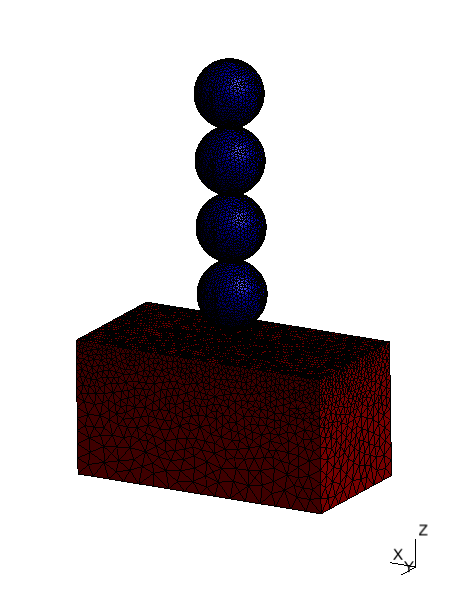
\includegraphics[height=3in]{geometry}
\caption{Geometry of cantilever and bead, truncated in the x direction and limited to tens of plasma wavelengths in depth. Here we show four distances of the bead from the cantilever in the z direction.}\label{fig:geo}
\end{figure}

\subsection{Proximity Force Approximation (PFA)}
\subsection{Expanded Proximity Force Approximation}
Most of this section taken from \citet{Dexp}, also see \citet{Bimonte12}

Normal energy of Casimir Effect:
$$
E_{pp}(z)=-\frac{\pi^2}{1440z^3}
$$

For $R>>a$:
$$
E_{C}\approx E_{PFA}=\int_{\Sigma}E_{pp}(z)d\sigma
$$

We don't expect this to hold much past this condition, but can use the derivative expansion to first order to obtain a slightly more accurate term. The formula for the derivative expansion in terms of some surface separation $z=\psi(\mathbf{x}_\parallel)$ is
$$
E_{DE}=-\frac{\pi^2}{1440}\int\frac{1}{\psi^3}\left(1+\frac{2}{3}(\partial_\alpha \psi)^2\right)d\mathbf{x}_\parallel
$$
and if we add in the correction factor $\eta_E(z)$ (see next section), we get
$$
E_{DE}=-\frac{\pi^2}{1440}\int\frac{\eta_E(\psi)}{\psi^3}\left(1+\frac{2}{3}(\partial_\alpha \psi)^2\right)d\mathbf{x}_\parallel
$$
which, given the complexity of $\eta_E$, is best evaluated numerically. We can parameterize the surface of a sphere as
$$
\psi_0(r)=R\left(1-\sqrt{1-\frac{r^2}{R^2}}\right)
$$
where the surface separation would be $\psi=a+\psi_0(r)$ and $a$ the minimal separation between sphere and plane. Given that the derivative with respect to $\theta$ is 0, the integral simplifies to
$$
E_{DE}=-\frac{2\pi^3}{1440}\int\frac{\eta_E(\psi)}{\psi^3}\left(1+\frac{2}{3}(\partial_r \psi)^2\right)dr
$$
and we can write, as well, 
$$
(\partial_r\psi)^2=R^2\left[-\frac{1}{2}\left(1-\frac{r^2}{R^2}\right)^{-1/2}\left(\frac{-2r}{R^2}\right)\right]^2=\frac{r^2}{R^2(1-\frac{r^2}{R^2})}=\frac{r^2}{R^2-r^2}=\left(\frac{R^2}{r^2}-1\right)^{-1}
$$
we can see that the derivative is undefined if we integrate to $R$, so as long as we integrate to $r_{limit}<R$ we should have a convergent integral; this shouldn't affect the accuracy given the $r^{-3}$ dependence. The effect of the derivative expansion correction in a perfectly conducting system can be seen below.

\begin{figure}[h]
\centering
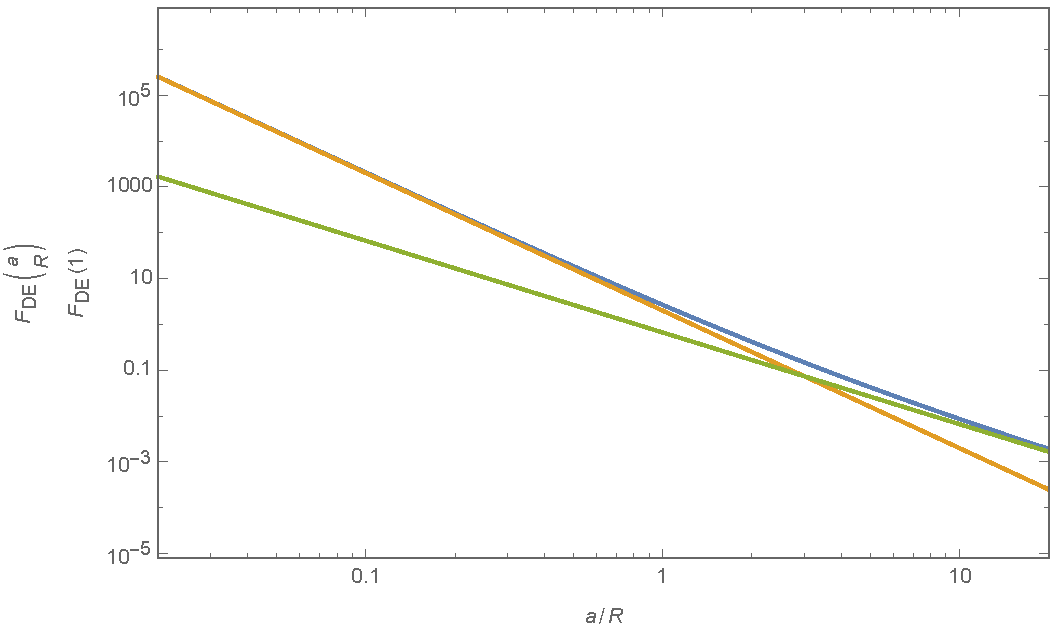
\includegraphics[width=5in]{PFAExpansion}
\caption{Illustration of the effect of the first order correction on the PFA; blue line shows expansion, orange line is PFA, green line is first order correction.}\label{fig:expansion}
\end{figure}

\citet{Bulgac} calculate the force between plane and sphere exactly, and compare to PFA. \citet{Durand} explore various temperature and geometry effects as a function of radius and separation. 

\section{Finite Conductivity Corrections}
\subsection{Dielectric Correction}
\citet{BeyondPFA,Lambrecht}: dielectric effects, non-perfect conductivity. The following mostly from \citet{Lambrecht}

The dielectric constant is large at frequencies smaller than the plasma frequency $\omega_p$, so corrections are more relevant at separations smaller than the plasma wavelength
$$
\lambda_p=\frac{2\pi c}{\omega_p}
$$
where
$$
\omega_p^2=\frac{Nq^2}{\epsilon_0m^*}=\frac{ZN_aq^2}{\epsilon_0m^*}=\frac{\rho q^2}{\epsilon_0m^*m_z}
$$
and in turn, $N$ is the number of conduction electrons per unit volume, $Z$ is the number of free electrons per atom (taken to just be $Z=1$), $N_a$ is the atomic number density, $q$ is the electron charge, and $m^*$ is effective electron mass, also taken to be 1 for Au though not necessarily for $\mathrm{SiO^2}$. We in turn calculate $N_a$ as the density $\rho$ divided by the atomic mass $m_Z$ for the species.

Thermal corrections relevant at distances larger than 
$$
\lambda_T=\frac{\hbar c}{k_B T}
$$
The reduction factor for the Casimir energy is given by
\begin{equation}
\eta_E=-\frac{180L^3}{c\pi^4}\int^{\infty}_{0}\kappa d\kappa\int^{c\kappa}_0\sum_{p=\parallel,\perp}\log{\left(1-r_{p,1}(i\omega,i\kappa)r_{p,2}(i\omega,i\kappa)e^{-2\kappa L}\right)}d\omega
\end{equation}
where $r_{p,i}(i\omega,i\kappa)$ is the reflection amplitude of surface $i$ for polarization $p$, where $i\omega$ is the imaginary frequency and $i\kappa$ is the imaginary wave vector along the longitudinal direction of the cavity, or the normal to the plane. The reflection coefficients for thick slabs are given by
\begin{align}
r_{\perp}&=-\frac{\sqrt{\omega^2(\epsilon(i\omega)-1)+c^2\kappa}-c\kappa}{\sqrt{\omega^2(\epsilon(i\omega)-1)+c^2\kappa}+c\kappa} \\
r_{\parallel}&=\frac{\sqrt{\omega^2(\epsilon(i\omega)-1)+c^2\kappa}-c\kappa\epsilon(i\omega)}{\sqrt{\omega^2(\epsilon(i\omega)-1)+c^2\kappa}+c\kappa\epsilon(i\omega)}
\end{align}

\citet{Lambrecht} suggest numerical integration over the range $10^{-4}$ to $10^{3}$ eV for distances 0.1 to 10 $\mu$m

\subsection{Expected accuracy}
We are limited by the validity of the proximity force approximation, which assumes the (roughly) Casimir forces are additive, which is known not to be the case, and assumes the sphere and plane are close enough such that the plane appears infinite and the curvature is relatively small. We include the first order correction to the PFA, which may not extend validity very far and still assumes the plane is long enough to be effectively infinite.

\section{Numerical Computation}



\pagebreak
\appendix
\section{Scuff-EM}
\section{Casimir Force Code}

\bibliographystyle{plainnat}
\bibliography{Casimir}

\end{document}  